\documentclass[a4paper,12pt]{article}
\usepackage[T2A]{fontenc}
\usepackage[utf8]{inputenc}
\usepackage[russian]{babel}
\usepackage{graphicx}
\usepackage{float}
\usepackage{subcaption}
\usepackage{amsmath, amssymb}
\usepackage{geometry}
\usepackage{amsmath}
\usepackage{tikz}
\usepackage{hyperref}
\geometry{top=2cm, bottom=2cm, left=3cm, right=1.5cm}

\begin{document}

\thispagestyle{empty}
\begin{center}
    \large
    Министерство науки и высшего образования Российской Федерации\\
    Федеральное государственное автономное образовательное учреждение\\
    высшего образования\\
    «Национальный исследовательский университет ИТМО»\\
    \vspace{5cm}
    \textbf{Отчёт по исследовательской работе № 1}\\
    \textbf{По предмету: Математический анализ и основы вычислений}\\
    \vspace{6cm}
    \begin{flushright}
        Выполнил работу:\\ Тиганов Вадим Игоревич\\
        \vspace{1cm}
        Академическая группа: \\ J3112\\
        \vspace{1cm}
        Вариант: \\18
    \end{flushright}
    \vspace{1cm}
    \vspace{3cm}
    \begin{center}
        Санкт-Петербург, 2025\\
    \end{center}
\end{center}

\newpage


\section{Ход работы}


\subsection{Задание 5}

Требуется:
Кривая задана как пересечение плоскостей. Задать ее уравнение
параметрически и вычислить длину.

\begin{equation}
    \begin{cases}
        &z^3 = 12x\\
        &2zy = 4\\
        &\frac{2}{3} \le x \le 18
        
    \end{cases}\,.
\end{equation}


\emph{Графическое изображение фигуры:}
\begin{figure}[H]
    \centering
    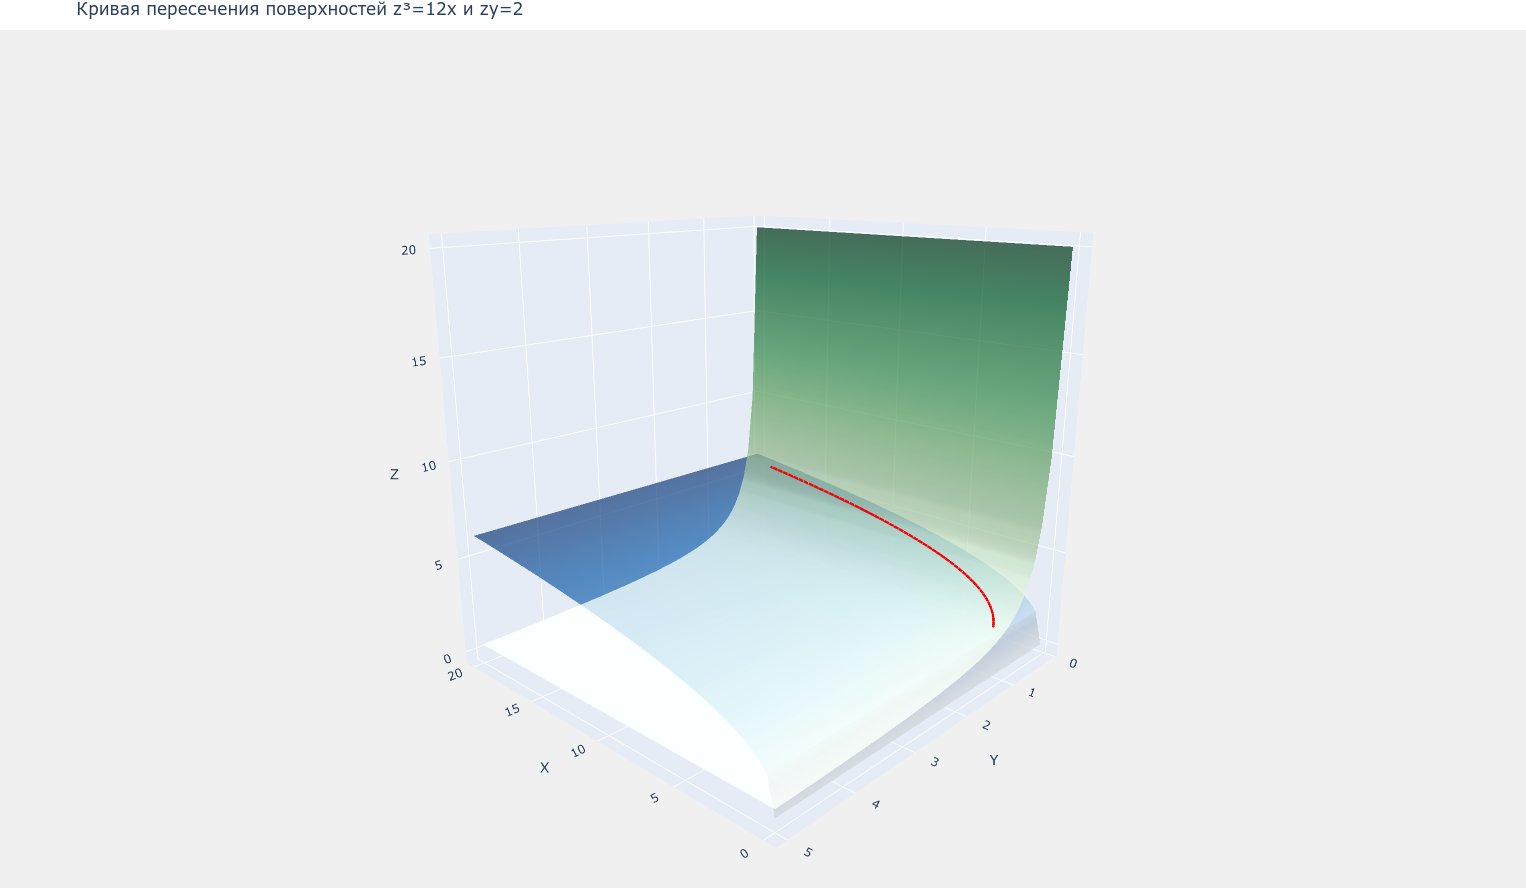
\includegraphics[width=0.9\linewidth]{../img/task5_plot.png}
    \label{fig:integral}
\end{figure}

\emph{Решение задачи:}

\begin{figure}[H]
    \centering
    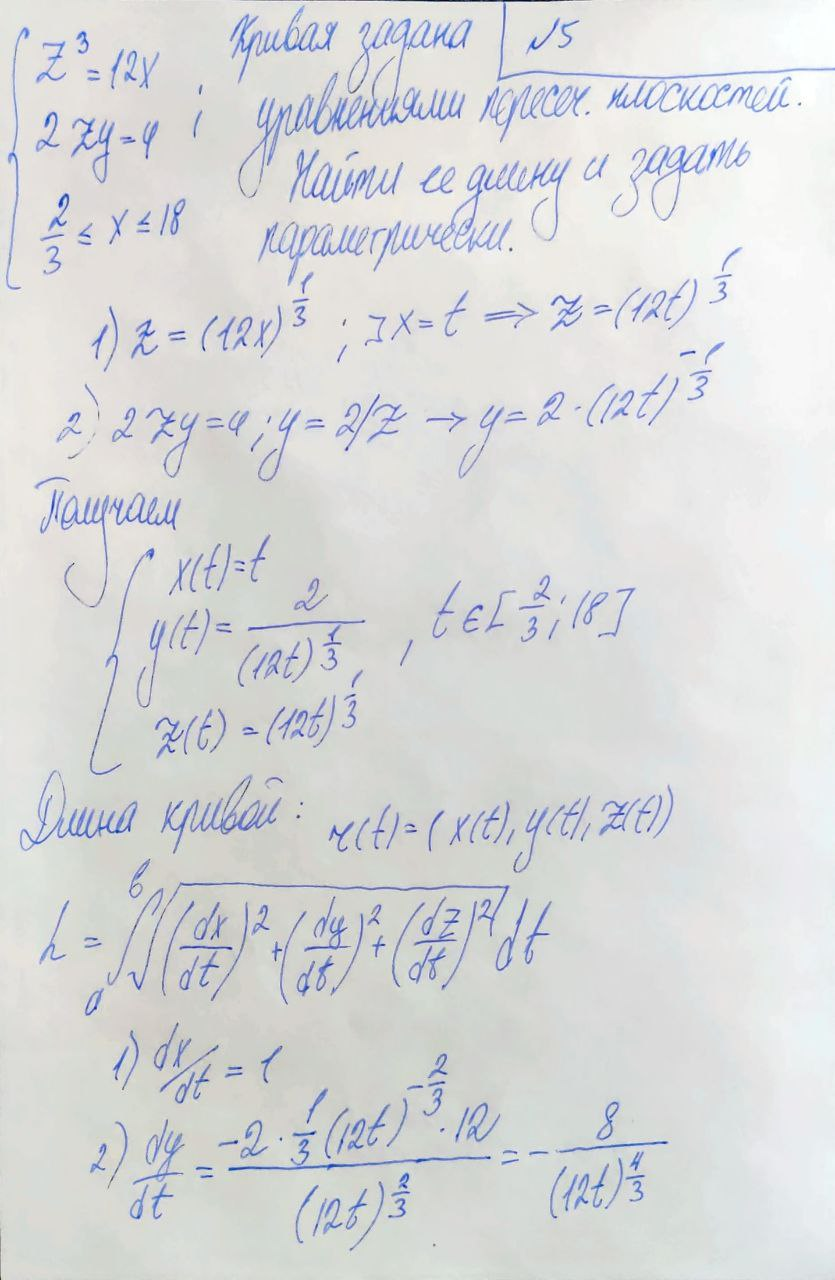
\includegraphics[width=0.9\linewidth]{../img/5_1.jpg}
    \label{fig:integral}
\end{figure}

\begin{figure}[H]
    \centering
    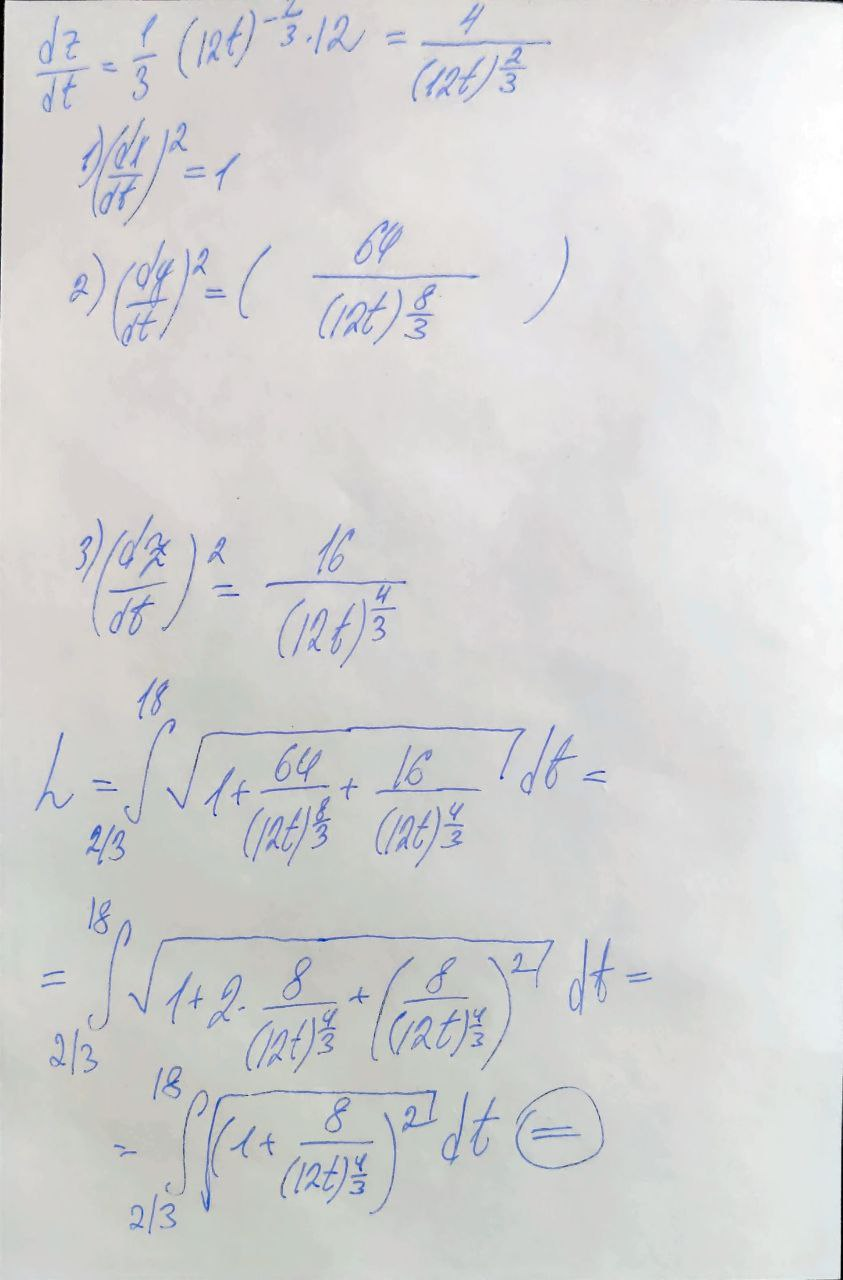
\includegraphics[width=0.9\linewidth]{../img/5_2.jpg}
    \label{fig:integral}
\end{figure}

\begin{figure}[H]
    \centering
    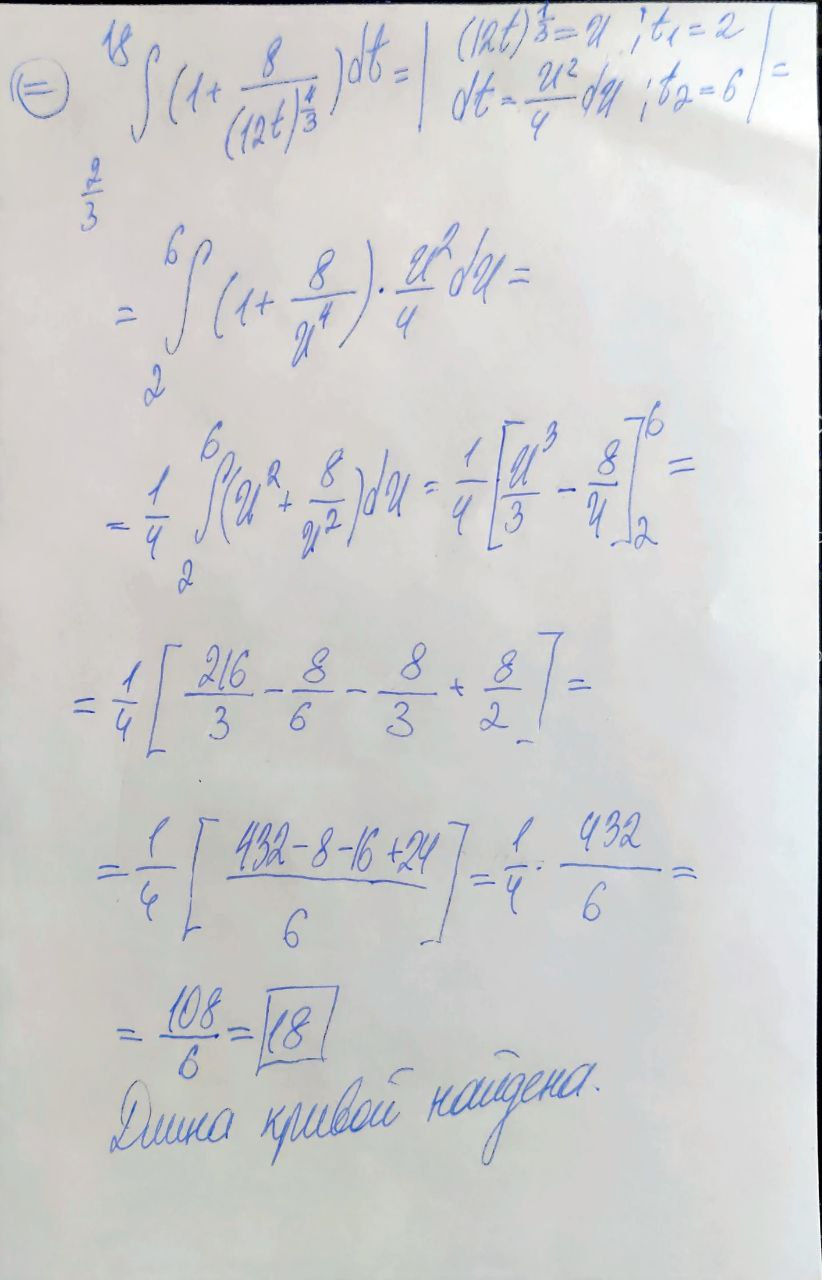
\includegraphics[width=0.9\linewidth]{../img/5_3.jpg}
    \label{fig:integral}
\end{figure}
\emph{Задача решена}, параметризовать удалось без каких-либо проблем, отрезок интегрирования
был дан по условию. Посчитал и получил ответ, проверял на \verb|Python|, ответ сошелся.

\end{document}